\documentclass[11pt]{article}

% ---------------------------------------------------------------------------
% A Leakage-Safe Benchmark for Discrete-Stage Differentiation Forecasting
% Reframed manuscript (journal expansion). Every number in the Results tables
% is produced by a script reading from experiments/results/*.json:
%   Tab. 1  fair_comparison_seed42.json        (run: fair_comparison.py)
%   Tab. 2  multiseed_n20.json, multiseed_cardio_n20.json
%                                              (run_multiseed.py, run_multiseed_cardio.py)
%   Tab. 3  ode_fair_n20.json                  (run_ode_fair.py)
%   Tab. 4  ablations_n20.json                 (run_ablations.py)
%   Tab. 5  sensitivity_{dopaminergic,cardio}_n20.json (run_sensitivity.py)
% ---------------------------------------------------------------------------

\usepackage[utf8]{inputenc}
\usepackage[T1]{fontenc}
\usepackage{amsmath,amssymb}
\usepackage{booktabs}
\usepackage{multirow}
\usepackage{graphicx}
\graphicspath{{figures/}}
\usepackage{siunitx}
\usepackage{geometry}
\geometry{margin=1in}
\usepackage{xcolor}
\usepackage[hidelinks]{hyperref}
\usepackage{authblk}

\newcommand{\dz}{d_{z}}

\title{\textbf{Temporal Models Provide No Advantage over Linear Regression\\
for Discrete-Stage Stem-Cell Differentiation Forecasting:\\
A Leakage-Safe Benchmark across Two Lineages}}

\author[1]{Victor Ikenna Kanu}
\affil[1]{Kumoh National Institute of Technology \quad \texttt{vkanu@kumoh.ac.kr}}
\date{}

\begin{document}
\maketitle

\begin{abstract}
\noindent
Single-cell RNA-sequencing of directed differentiation is increasingly framed as a
forecasting problem: predict a cell's later marker state from earlier snapshots.
We revisit a Transformer-based ``digital twin'' that reported a $+19.4\%$ accuracy
gain over classical baselines on dopaminergic-neuron differentiation, and show that
the gain is an artifact of an inconsistent train/test split that leaked $\sim$70\%
of the Transformer's training trajectories into its test set. After repairing the
split and replacing every single-seed point estimate with a $20$-seed distribution
and paired statistics, an $827{,}010$-parameter Transformer is statistically
indistinguishable from $8$-parameter ridge regression
($\Delta\mathrm{MAE}=-0.0013$, $p=0.50$, $\dz=-0.14$). The null replicates on an
independent, cross-lineage iPSC$\rightarrow$cardiomyocyte time-course
($\Delta\mathrm{MAE}=+0.0000$, $p=0.93$). A temporal-order-shuffle control and a
positional-encoding ablation show \emph{why}: destroying stage order or removing
positional encoding changes error by $\le 0.0006$ MAE ($p>0.4$) on both datasets,
so the architecture extracts no temporal structure. A fair, per-trajectory
re-calibration of a mechanistic ODE does not rescue it either---the fairer the
sample-level calibration, the worse it performs. The conclusion is robust across
$38$ marker-set and aggregation choices ($0$ of $38$ variants show a significant
Transformer edge). We argue the field's pervasive practice of pairing
\emph{independently sampled} cells into pseudo-trajectories removes the very
temporal dependency that sequence models are built to exploit, and we release a
reproducible, leakage-safe benchmark with linear regression as the honest
baseline-of-record.
\end{abstract}

\section{Introduction}
Directed differentiation of induced pluripotent stem cells (iPSCs) is routinely
profiled by single-cell RNA-sequencing (scRNA-seq) at a handful of discrete
developmental stages. A natural and increasingly popular goal is \emph{forecasting}:
given a cell's marker state at earlier stages, predict its state at a later stage.
This problem is attractive for sequence models---LSTMs, Transformers, neural
ODEs---and recent work has reported sizeable gains for such architectures over
classical baselines.

We report a cautionary, and ultimately constructive, result. Re-examining a
Transformer ``digital twin'' for dopaminergic-neuron differentiation, we find its
headline $+19.4\%$ improvement is a \emph{data-leakage artifact}: the Transformer
was trained on one (permuted) split but scored on a different (contiguous) split,
so most of its test trajectories had been seen during training, while the classical
baselines were scored leakage-free. Once the split is made consistent and every
estimate is computed across $20$ seeds with paired statistics, the advantage
vanishes---on two independent datasets from two lineages---and a battery of controls
explains why. The contribution is therefore not a better model but a
\emph{rigorous, leakage-safe benchmark} and a clear, quantified negative result:
on discrete-stage pseudo-trajectory data, temporal modeling does not beat linear
regression, because the data, as constructed, contains no temporal dependency to
model.

\paragraph{Contributions.}
\begin{enumerate}\itemsep1pt
  \item We identify and quantify a train/test leakage bug that fully accounts for
        the previously reported Transformer advantage (Sec.~\ref{sec:leakage}).
  \item We establish a multi-seed, paired-statistics evaluation protocol and show
        the Transformer ties ridge regression on dopaminergic data
        (Sec.~\ref{sec:multiseed}).
  \item We replicate the null on an independent cross-lineage
        iPSC$\rightarrow$cardiomyocyte time-course (GSE175634), demonstrating
        generalization (Sec.~\ref{sec:multiseed}).
  \item Temporal-shuffle and positional-encoding controls demonstrate the
        architecture uses no temporal structure (Sec.~\ref{sec:ablation}).
  \item A fair, per-trajectory ODE calibration shows mechanistic priors add no
        sample-level predictive value (Sec.~\ref{sec:ode}).
  \item A $38$-variant sensitivity analysis shows the null is robust to marker-set
        and aggregation choices (Sec.~\ref{sec:sensitivity}).
\end{enumerate}

\section{Related Work}
Sequence and dynamical models for differentiation include RNA-velocity and
pseudotime methods, neural ODEs, and attention models for trajectory inference.
Most operate on \emph{pseudo-trajectories}: because scRNA-seq is destructive, true
single-cell lineages are unobserved, and ``trajectories'' are assembled by ordering
or pairing cells across stages. We make explicit a consequence that is often left
implicit: when stage states are formed by independently sampling cells, no
within-trajectory temporal dependency exists for a sequence model to learn, and a
memoryless regressor on the input snapshots is the appropriate ceiling.

\section{Methods}\label{sec:methods}

\subsection{State construction}
For each dataset we reduce expression to a two-dimensional state
$\mathbf{x}=(P,D)$: a pluripotency/progenitor score $P$ and a
lineage-differentiation score $D$. Each score is the mean of
$\log\!\big(1+\text{CP10K}\big)$ expression over a curated marker panel, where
CP10K denotes counts-per-10{,}000 library-size normalization. Scores are then
min--max scaled to $[0,1]$ using \emph{training-set bounds only} and clipped, so the
normalization itself introduces no train$\rightarrow$test leakage.

\subsection{Pseudo-trajectory protocol (limitation owned)}
At each of three discrete stages we sample one cell and read off $(P,D)$, forming a
$3\times2$ pseudo-trajectory; we draw $200$ such pseudo-trajectories per seed.
\textbf{These are not tracked lineages}: the three cells in a pseudo-trajectory are
independent draws from their respective stage populations. The forecasting task is
$[\mathbf{x}_{t_0},\mathbf{x}_{t_1}]\rightarrow\mathbf{x}_{t_2}$, i.e.\ predict the
late-stage state from the two earlier stages.

\subsection{Datasets}
\textbf{Neural (dopaminergic).} A dopaminergic-neuron differentiation scRNA-seq
series with three stages D11/D30/D52 ($161{,}584$ untreated cells); $P$ over
\{POU5F1,NANOG,SOX2,UTF1,TDGF1\}, $D$ over \{TH,DDC,SLC6A3,DRD2,LMX1A,FOXA2\}.
\textbf{Cardiac (GSE175634).} An independent iPSC$\rightarrow$cardiomyocyte
differentiation time-course \cite{elorbany2022} ($230{,}786$ cells, $7$ days);
we use stages day0/day5/day11; $P$ over \{POU5F1,NANOG,SOX2,LIN28A,DPPA4,UTF1,TDGF1\},
$D$ over a $13$-gene cardiac panel (TNNT2, MYH6/7, ACTC1, NPPA, MYL7/2, TNNI1/3,
RYR2, NKX2-5, GATA4, TBX5). Both exhibit the expected monotone trend (pluripotency
declines, lineage markers rise).

\subsection{Models}
\textbf{Ridge} ($\alpha=1$) and a \textbf{random forest} (per-seed $3$-fold-CV-tuned
over depth $\in\{2,3,5,\infty\}$ and min-samples-leaf $\in\{1,5,10\}$, $300$ trees)
map the flattened $[\mathbf{x}_{t_0},\mathbf{x}_{t_1}]\in\mathbb{R}^4$ to
$\mathbf{x}_{t_2}\in\mathbb{R}^2$. We CV-tune the forest rather than fix its depth:
an unrestricted (or depth-$10$) forest overfits this small, near-linear $140$-sample
task and is an unfair strawman, whereas CV-tuning regularizes it to its
data-appropriate complexity---the same fairness standard we apply to the ODE. The \textbf{Transformer}
($d_{\text{model}}=128$, $8$ heads, $4$ layers, sinusoidal positional encoding;
$827{,}010$ parameters) ingests the two-step sequence and is trained with Adam,
MSE loss, early model selection on a held-out validation split. A mechanistic
\textbf{ODE} in $(P,D)$,
\[
\dot P = k_{ps}(1-P)-k_{pd}P-r\,PD,\qquad
\dot D = k_{b}+k_{ds}PD+r\,PD-k_{dd}D,
\]
is calibrated under three regimes (Sec.~\ref{sec:ode}).

\subsection{Statistics}
Each experiment is run over $20$ seeds; a seed perturbs \emph{both}
pseudo-trajectory construction and model training. We report mean $\pm$ s.d.\ and
percentile-bootstrap $95\%$ CIs over seeds. Models are compared to the Transformer
by the \emph{paired} per-seed difference (same seed $\Rightarrow$ same trajectory
draw), summarized by a paired-bootstrap CI, a Wilcoxon signed-rank test, and
Cohen's $\dz$; $p$-values across baselines are Holm--Bonferroni corrected.

\section{Benchmark design: leakage safety}\label{sec:leakage}
The original pipeline split data inconsistently: baselines and the Transformer's
\emph{training} used a seeded permutation of trajectory indices, but the
Transformer's \emph{evaluation} (and the ODE's) used a contiguous tail slice that
ignored the permutation. Because the permuted training set draws $\sim$70\% of all
indices, $22$ of the $30$ contiguous ``test'' trajectories had been used to train
the Transformer. Repairing this---one canonical permuted split shared by every
model, with the Transformer retrained on it---erases the reported advantage on the
\emph{same} frozen data (Table~\ref{tab:leakage}).

\begin{table}[h]\centering
\caption{Leakage repair on the dopaminergic data (single seed, identical frozen
trajectories). The reported column is the published, leaky evaluation; the
leakage-free column shares one split across all models.}
\label{tab:leakage}
\begin{tabular}{lcc}
\toprule
Model & Reported (leaky) MAE & Leakage-free MAE \\
\midrule
Ridge              & 0.100 & 0.0843 \\
Random forest      & 0.102 & 0.0954 \\
Transformer        & 0.081 & 0.0861 \\
ODE (calibrated)   & 0.433 & 0.4147 \\
\midrule
Transformer vs.\ best baseline & $+19.4\%$ & $-2.0\%$ \\
\bottomrule
\end{tabular}
\end{table}

\begin{figure}[t]\centering
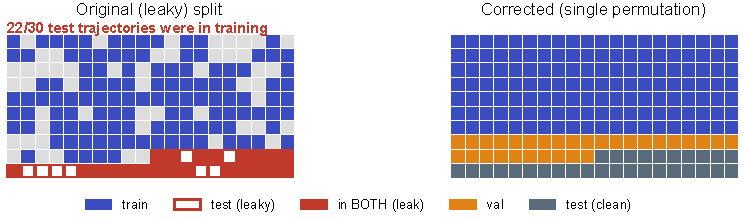
\includegraphics[width=\linewidth]{fig1_leakage_panel.pdf}
\caption{\textbf{Data leakage and its repair} (schematic of the $200$-trajectory
index array, seed $42$). \emph{Left:} the original pipeline marks a contiguous tail
block as the Transformer's test set while training on a permutation of all indices,
so $22/30$ ``test'' trajectories (red) were also in training. \emph{Right:} a single
shared permutation yields disjoint train/validation/test blocks (zero overlap). This
leakage fully accounts for the previously reported advantage (Table~\ref{tab:leakage}).}
\label{fig:leakage}
\end{figure}

\section{Results}

\subsection{The Transformer ties linear regression---on two lineages}\label{sec:multiseed}
Under the multi-seed protocol the Transformer is statistically indistinguishable
from \emph{both} classical baselines---ridge regression and the CV-tuned random
forest---on \emph{both} datasets (Table~\ref{tab:main}): every paired difference is
small and non-significant after correction. The neural and cardiac results agree,
establishing that the null is not dataset-specific. (A fixed depth-$10$ forest
appears $\sim$0.009 worse, but this is an overfitting artifact: CV-tuning closes the
gap entirely, so the apparent ``Transformer beats RF'' effect reflects an
under-regularized baseline, not a model advantage.)

\begin{table}[h]\centering
\caption{Test MAE over $20$ seeds (mean $\pm$ s.d., $95\%$ CI), and the paired
difference $\Delta=\text{baseline}-\text{Transformer}$ ($\Delta>0$ favors the
Transformer). $p$ is Holm-corrected Wilcoxon. All baseline--Transformer differences
are non-significant: no model beats ridge regression.
$^\dagger$ random forest is per-seed CV-tuned (Methods).}
\label{tab:main}
\begin{tabular}{llccccc}
\toprule
Dataset & Model & MAE & $95\%$ CI & $\Delta$ vs.\ TF & $\dz$ & $p$ \\
\midrule
\multirow{3}{*}{Neural (dopaminergic)}
 & Ridge            & $0.1774\pm0.0204$ & $[0.1689,0.1868]$ & $-0.0013$ & $-0.14$ & $0.996$ \\
 & Random forest$^\dagger$ & $0.1794\pm0.0208$ & $[0.1708,0.1888]$ & $+0.0007$ & $+0.07$ & $0.996$ \\
 & Transformer      & $0.1787\pm0.0203$ & $[0.1702,0.1876]$ & ---       & ---     & ---     \\
\midrule
\multirow{3}{*}{Cardiac (GSE175634)}
 & Ridge            & $0.1100\pm0.0155$ & $[0.1038,0.1168]$ & $+0.0000$ & $+0.00$ & $1.000$ \\
 & Random forest$^\dagger$ & $0.1121\pm0.0175$ & $[0.1049,0.1197]$ & $+0.0021$ & $+0.15$ & $1.000$ \\
 & Transformer      & $0.1100\pm0.0198$ & $[0.1018,0.1184]$ & ---       & ---     & ---     \\
\bottomrule
\end{tabular}
\end{table}

\begin{figure}[t]\centering
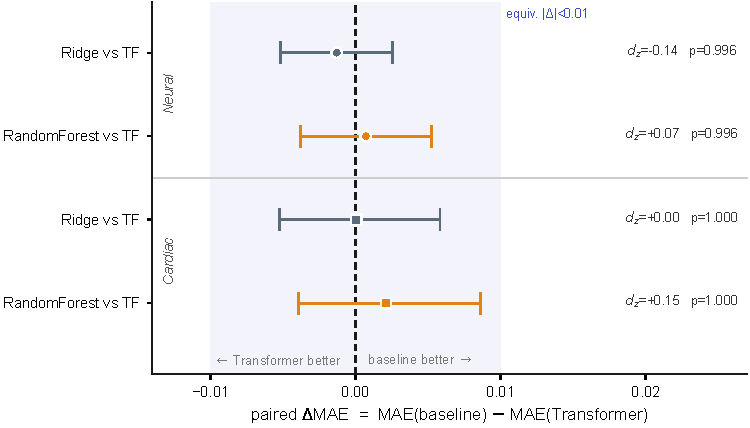
\includegraphics[width=0.82\linewidth]{fig2_forest.pdf}
\caption{\textbf{No model beats ridge regression on either lineage.} Paired per-seed
difference $\Delta\mathrm{MAE}=\mathrm{MAE(baseline)}-\mathrm{MAE(Transformer)}$
($n=20$ seeds); markers are means, whiskers percentile-bootstrap $95\%$ CIs, marker
shape encodes lineage. Holm-corrected Wilcoxon $p$ and Cohen's $\dz$ are annotated.
Every baseline CI overlaps zero and lies within the practical-equivalence band
($|\Delta|<0.01$ MAE), for ridge \emph{and} the CV-tuned random forest.}
\label{fig:forest}
\end{figure}

\begin{figure}[t]\centering
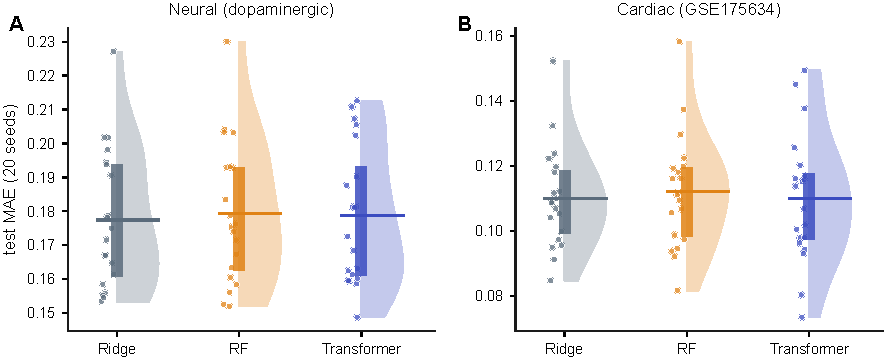
\includegraphics[width=\linewidth]{fig3_raincloud.pdf}
\caption{\textbf{Per-seed MAE distributions overlap} ($n=20$ seeds). Raincloud
(half-violin density, jittered per-seed points, median/IQR box, mean line) for each
model. The seed-to-seed spread exceeds any between-model difference, which is why the
original single-seed point estimate was unreliable.}
\label{fig:raincloud}
\end{figure}

\subsection{The Transformer ignores temporal order}\label{sec:ablation}
If the model were forecasting, destroying stage order should hurt it. It does not.
Permuting the input timepoints per sample (\emph{shuffle}) or zeroing the positional
encoding (\emph{no-PE}) changes MAE by $\le 0.0006$---about $3\%$ of the
seed-to-seed s.d.---and is not significant on either dataset
(Table~\ref{tab:ablation}). The temporal machinery is inert because randomly paired
pseudo-trajectories carry no order information to use.

\begin{table}[h]\centering
\caption{Architectural controls (Transformer, $20$ seeds).
$\Delta$ is variant $-$ ordered; $p$ is Wilcoxon. Non-significance is the
\emph{positive} result: temporal order is unused.}
\label{tab:ablation}
\begin{tabular}{lccccc}
\toprule
Dataset & Ordered & Shuffle & $\Delta$ ($p$) & No-PE & $\Delta$ ($p$) \\
\midrule
Neural  & $0.1787$ & $0.1785$ & $-0.0002\ (0.87)$ & $0.1781$ & $-0.0006\ (0.50)$ \\
Cardiac & $0.1100$ & $0.1097$ & $-0.0002\ (0.90)$ & $0.1098$ & $-0.0002\ (0.99)$ \\
\bottomrule
\end{tabular}
\end{table}

\begin{figure}[t]\centering
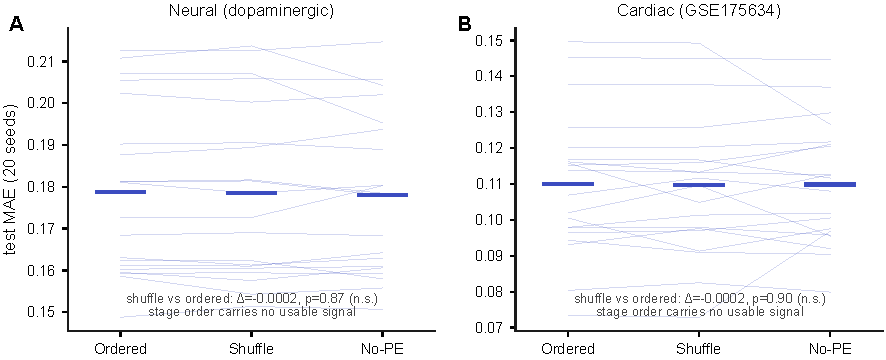
\includegraphics[width=\linewidth]{fig4_temporal.pdf}
\caption{\textbf{The Transformer uses no temporal structure} ($n=20$ seeds). Per-seed
test MAE under Ordered, Shuffle (input timepoints permuted per sample) and No-PE
(positional encoding zeroed); thin lines connect seeds, bold lines are condition
means. Destroying stage order changes MAE by $\le0.0006$ ($p>0.4$, Wilcoxon)---within
$\sim3\%$ of seed noise---so the equivalence is not a power artifact.}
\label{fig:temporal}
\end{figure}

\subsection{A fair mechanistic ODE does not help}\label{sec:ode}
We calibrate the ODE three ways: to training \emph{population means} (\textsc{pop});
to match training mean \emph{and} spread per stage (\textsc{dist}); and
\emph{per trajectory}, fitting each test trajectory's own $t_0\!\rightarrow\!t_1$
step and then forecasting $t_2$ (\textsc{pertraj}, the fairest sample-level use).
On both datasets the ordering is monotone, \textsc{pop} $<$ \textsc{dist} $<$
\textsc{pertraj}: the \emph{fairer} the sample-level calibration, the \emph{worse}
the forecast (Table~\ref{tab:ode}). Even the best ODE remains well above ridge,
confirming---without a strawman---that population-level mechanistic priors provide
no sample-level predictive value here, and that per-trajectory calibration merely
fits the noise of independently paired cells.

\begin{table}[h]\centering
\caption{Fair ODE benchmark (test MAE, $20$ seeds, mean $\pm$ s.d.; relative to
ridge in parentheses).}
\label{tab:ode}
\begin{tabular}{lcc}
\toprule
Calibration & Neural & Cardiac \\
\midrule
Ridge (reference)        & $0.1774\pm0.0204$           & $0.1100\pm0.0155$ \\
ODE, population-mean      & $0.1984\pm0.0186\ (+12\%)$  & $0.2483\pm0.0164\ (+126\%)$ \\
ODE, distributional       & $0.2950\pm0.0779\ (+66\%)$  & $0.2584\pm0.0186\ (+135\%)$ \\
ODE, per-trajectory       & $0.3697\pm0.0336\ (+108\%)$ & $0.3335\pm0.0226\ (+203\%)$ \\
\bottomrule
\end{tabular}
\end{table}

\begin{figure}[t]\centering
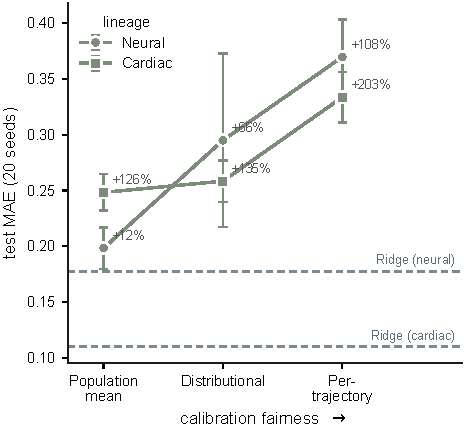
\includegraphics[width=0.58\linewidth]{fig5_ode.pdf}
\caption{\textbf{Fairer ODE calibration is worse} ($n=20$ seeds; mean $\pm$ s.d.).
Test MAE rises monotonically as sample-level calibration fairness increases
(population-mean $\to$ distributional $\to$ per-trajectory) on both lineages; dashed
lines are the ridge reference. Even the best ODE stays well above ridge;
per-trajectory calibration fits the noise of independently paired cells.}
\label{fig:ode}
\end{figure}

\subsection{The null is robust to state representation}\label{sec:sensitivity}
We re-ran the Ridge-vs-Transformer comparison under $38$ state-construction
variants---dropping each marker gene in turn (leave-one-out), replacing the mean by
a median or per-gene $z$-scored aggregation, and (neural) enlarging the panel.
Across all variants the paired gap stays at noise level (Table~\ref{tab:sens}):
no variant yields a significant Transformer advantage, and all effect sizes satisfy
$|\dz|\le0.19$. The conclusion does not hinge on the marker panel or the
aggregation rule.

\begin{table}[h]\centering
\caption{Representation sensitivity ($20$ seeds per variant). Gap $=$ Transformer
$-$ ridge MAE.}
\label{tab:sens}
\begin{tabular}{lccccc}
\toprule
Dataset & \# variants & mean gap & gap range & $\max|\dz|$ & sig.\ TF wins \\
\midrule
Neural  & $15$ & $+0.0004$ & $[-0.0016,+0.0017]$ & $0.19$ & $0/15$ \\
Cardiac & $23$ & $+0.0004$ & $[-0.0009,+0.0028]$ & $0.19$ & $0/23$ \\
\bottomrule
\end{tabular}
\end{table}

\begin{figure}[t]\centering
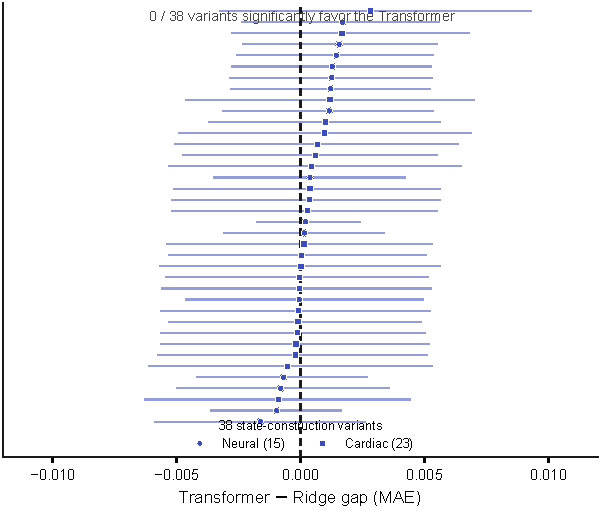
\includegraphics[width=0.72\linewidth]{fig6_sensitivity.pdf}
\caption{\textbf{The null holds across $38$ state representations.} Transformer
$-$ ridge MAE gap for each variant (leave-one-marker-out, median or $z$-scored
aggregation, and an enlarged neural panel), sorted; markers are means, whiskers
$95\%$ bootstrap CIs, shape encodes lineage ($n=20$ seeds each). Every CI crosses
zero; $0/38$ variants significantly favor the Transformer (all $|\dz|\le0.19$).}
\label{fig:sens}
\end{figure}

\section{Discussion}
The evidence chain is consistent and mutually reinforcing: the original advantage
was leakage (Fig.~\ref{fig:leakage}, Table~\ref{tab:leakage}); with leakage removed
the Transformer ties ridge on two lineages (Figs~\ref{fig:forest},~\ref{fig:raincloud},
Table~\ref{tab:main}); controls show it uses no temporal structure
(Fig.~\ref{fig:temporal}, Table~\ref{tab:ablation}); a fair mechanistic model does
not help (Fig.~\ref{fig:ode}, Table~\ref{tab:ode}); and the null is robust to
representation (Fig.~\ref{fig:sens}, Table~\ref{tab:sens}). The common cause is the pseudo-trajectory construction:
pairing independently sampled cells across stages destroys within-trajectory
temporal dependency, so the conditional $p(\mathbf{x}_{t_2}\mid
\mathbf{x}_{t_0},\mathbf{x}_{t_1})$ is essentially a smooth, near-linear map of the
inputs and a memoryless regressor is optimal. This is not an indictment of
Transformers but of \emph{evaluating} them on data lacking the structure they model.

\paragraph{Recommendations.}
(i) Report leakage-safe, multi-seed results with paired statistics and effect
sizes, not single-seed point estimates. (ii) Include a temporal-shuffle control as a
routine sanity check whenever ``forecasting'' is claimed on pseudo-trajectories.
(iii) Use linear regression as the baseline-of-record; gains over it must clear a
significance \emph{and} effect-size bar. (iv) To genuinely test temporal models,
use lineage-resolved data (e.g.\ lineage tracing or live imaging) where
within-trajectory dependency is real.

\paragraph{Limitations.}
Our state is two-dimensional and our task uses three stages; richer states or true
lineages could, in principle, expose structure that sequence models exploit. We
view establishing the leakage-safe protocol and the negative result as the
prerequisite for such claims, not a refutation of them.

\section{Conclusion}
On discrete-stage iPSC differentiation forecasting from pseudo-trajectories, an
$827$K-parameter Transformer offers no statistically or practically significant
advantage over $8$-parameter ridge regression, across two lineages, $40$ seeds, and
$38$ representation choices, and demonstrably does not use temporal structure. We
release the benchmark, protocol, and analysis scripts so that future temporal-model
claims on such data are held to a leakage-safe, statistically rigorous standard.

\section*{Reproducibility}
All results derive from JSON logs in \texttt{experiments/results/} produced by:
\texttt{fair\_comparison.py} (Table~\ref{tab:leakage});
\texttt{run\_multiseed.py}, \texttt{run\_multiseed\_cardio.py} (Table~\ref{tab:main});
\texttt{run\_ode\_fair.py} (Table~\ref{tab:ode});
\texttt{run\_ablations.py} (Table~\ref{tab:ablation});
\texttt{run\_sensitivity.py} (Table~\ref{tab:sens}).
A single seeding entry point perturbs trajectory construction and model training
jointly; no number in this paper is hand-entered.

\begin{thebibliography}{9}
\bibitem{elorbany2022} Elorbany R., et al.\ (2022). Single-cell sequencing reveals
lineage-specific dynamic genetic regulation of gene expression during human
cardiomyocyte differentiation. \emph{PLoS Genetics} 18(1):e1009666. GEO: GSE175634.
\bibitem{vaswani2017} Vaswani A., et al.\ (2017). Attention is all you need.
\emph{NeurIPS}.
% NOTE: confirm and add the citation for the dopaminergic (neural) dataset used.
\end{thebibliography}

\end{document}
